%% РУССКОЕ ЗЕРКАЛО дополнительных материалов для AAAI-27 — ДЛЯ ПРОВЕРКИ, НЕ ДЛЯ ПОДАЧИ.
%% Шаблон AAAI (aaai2027) запрещает кириллицу в тексте, поэтому это зеркало собрано
%% на обычном двухколоночном article + babel(russian) + tempora (как в журнальной RU-версии).
%% Содержание зеркалит ../en/supplement.tex. Не анонимно (зеркало не подаётся в AAAI).
%% Сборка: pdflatex supplement_ru ; bibtex supplement_ru ; pdflatex supplement_ru ; pdflatex supplement_ru
\documentclass[10pt,twocolumn,letterpaper]{article}

\usepackage[T2A]{fontenc}
\usepackage[utf8]{inputenc}
\usepackage[english,russian]{babel}
\usepackage{tempora}                       % Times-клон с полной кириллицей (жирная/курсив в T2A)
\usepackage[protrusion=true,expansion=false]{microtype}
\usepackage[letterpaper,margin=0.75in]{geometry}
\setlength{\columnsep}{0.3in}
\usepackage{graphicx}
\graphicspath{{../../../shared/figures/}}
\usepackage{amsmath,amssymb}
\usepackage{booktabs}
\usepackage{array}
\usepackage{cite}

\setcounter{secnumdepth}{2}

\begin{document}
\twocolumn[{%
  \begin{center}
  \LARGE\bfseries Дополнительные материалы:\\ Кросс-возрастная верификация лиц\\ по добытым парам одного человека из соцсетей\\[0.5em]
  \large\mdseries Д.~Ф.~Вольхин \quad И.~С.~Копылов\\[0.25em]
  \normalsize НИУ «Высшая школа экономики», Москва, Россия\quad\texttt{deneal123@mail.ru}
  \end{center}
  \vspace{0.6em}
  \begin{center}\small\itshape
  Русское зеркало для проверки. Это \textbf{не} материал для подачи в AAAI: шаблон AAAI
  запрещает кириллицу в тексте, поэтому официальная подача — англоязычная (\texttt{../en/}).
  \end{center}
  \vspace{1.2em}
}]

\noindent В этом приложении приведены контроли, аудиты, полные таблицы операционных точек, а также
карточки данных и модели, перенесённые из основной статьи ради места. Нумерация здесь внутренняя для
данного документа; ссылки на основную статью даются по названию. Все эксперименты используют очищенные
данные и тот же протокол атрибуции со слабым backbone, описанный в основной статье.

\section{Расширенное позиционирование среди связанных работ}\label{sup:positioning}
Табл.~\ref{tab:positioning} позиционирует наш естественно-супервизируемый источник относительно
дискриминативной, контрастивной линий и линии синтетического старения. Общий мотив в том, что
предшествующие методы зависят от \emph{ручных} меток личности и/или возраста либо от синтезированных
кросс-возрастных образцов, тогда как мы добываем структуру «один пост $=$ один человек в разном
возрасте» как генератор позитивных пар без меток.

\begin{table*}[t]
\centering
\small
\begin{tabular}{@{}p{0.15\textwidth}p{0.15\textwidth}p{0.30\textwidth}p{0.30\textwidth}@{}}
\toprule
Работа & Супервизия & Механизм & Наше отличие \\
\midrule
OE-CNN (2018)~\cite{wang2018oecnn} & размеч.\ id$+$возраст & ортогональная декомпозиция признаков & нет ручных меток id/возраста, не декомпозиция \\
DAL (2019)~\cite{wang2019dal} & размеч.\ id$+$возраст & adversarial-факторизация id/возраста & добытые пары $+$ проще цель \\
MTLFace (2021)~\cite{huang2021mtlface} & размеч.\ id$+$возраст & распознавание $+$ синтез возраста (multi-task) & слабее конвейер; новый источник супервизии \\
CACon (2023)~\cite{wang2024cacon} & полу-супер.\ $+$ синтетика & контрастив на синтезир.\ кросс-возрасте & реальные добытые пары $>$ синтетич.\ старение \\
Synthetic Ageing (2024)~\cite{yao2024synthageing} & синтетика & обучение на состаренных изображениях & мы делаем \emph{реальный} майнинг тезисом \\
OrdCon (2025)~\cite{wang2025ordcon} & возраст-упоряд.\ контрастив & order-enhanced признаки & добываем естеств.\ пары, без явного порядка возраста \\
\bottomrule
\end{tabular}
\caption{Позиционирование относительно предшествующих работ.}
\label{tab:positioning}
\end{table*}

\section{Данные и детали аудита}\label{sup:audit}
\textbf{Извлечение возраста.} По всем 33{,}697 мультифото-постам с подписями LLM и regex согласуются на
72.8\% (табл.~\ref{tab:age}); LLM дополнительно заполняет ещё 10.8\%, пропущенных regex, и предпочтителен
в большинстве из 13.8\% расхождений (он не читает календарные годы или разрывы как возраст).

\begin{table}[t]
\centering
\small
\begin{tabular}{@{}lrr@{}}
\toprule
Категория & $n$ & Доля \\
\midrule
Согласие (те же возрасты или оба пусты) & 24{,}531 & 72.8\% \\
LLM заполнил (regex пропустил) & 3{,}656 & 10.8\% \\
Расхождение возраста & 4{,}658 & 13.8\% \\
LLM пропустил (regex нашёл) & 852 & 2.5\% \\
\bottomrule
\end{tabular}
\caption{Аудит извлечения возраста: LLM против regex (33{,}697 мультифото-постов с подписями).}
\label{tab:age}
\end{table}

\textbf{Целостность групп.} Кластеризация по личностям уже отделила большинство многолюдных постов;
LLM-проход по целостности групп (табл.~\ref{tab:integrity}) помечает лишь 421 группу как шумную
(несколько людей / мем).

\begin{table}[t]
\centering
\small
\begin{tabular}{@{}lrr@{}}
\toprule
Категория & $n$ & Доля \\
\midrule
Один (один человек сквозь возраст) & 31{,}275 & 92.8\% \\
Несколько людей (разные люди) & 2{,}034 & 6.0\% \\
Неизвестно & 336 & 1.0\% \\
Мем / коллаж & 52 & 0.2\% \\
\bottomrule
\end{tabular}
\caption{LLM-классификация целостности групп (33{,}697 постов).}
\label{tab:integrity}
\end{table}

\textbf{Устойчивость к порогу дедупа.} Сокращение числа позитивов на $-$52\% от удаления near-duplicate —
не артефакт порога 0.97: оно стабильно в диапазоне 0.93--0.97 и деградирует лишь на очень строгом 0.99
(табл.~\ref{tab:dedupsens}).

\begin{table}[t]
\centering
\small
\begin{tabular}{@{}lrrr@{}}
\toprule
Дедуп cos & Near-dup лиц & Позитивов & Сокращение \\
\midrule
0.93 & 8{,}653 & 31{,}304 & $-$52.5\% \\
0.95 & 8{,}564 & 31{,}611 & $-$52.0\% \\
0.97 (исп.) & 8{,}304 & 32{,}360 & $-$50.9\% \\
0.99 & 6{,}274 & 38{,}565 & $-$41.5\% \\
\bottomrule
\end{tabular}
\caption{Чувствительность к порогу дедупа (только удаление near-duplicate, на группах до очистки; прун
целостности групп убирает ещё ${\approx}500$ до итоговых 31{,}865).}
\label{tab:dedupsens}
\end{table}

\textbf{Небольшая ручная валидация.} Один аннотатор выборочно проверил автоматический конвейер
(табл.~\ref{tab:humanval}). С одним аннотатором и без межаннотаторной $\kappa$ это \emph{поддерживает},
но не \emph{сертифицирует} супервизию; масштабный многоаннотаторный аудит остаётся вне наших ресурсов,
поэтому остаточный шум меток честно отмечен как ограничение. Выборки взяты из очищенного корпуса и не
использовались для настройки порогов или правил фильтрации.

\begin{table}[t]
\centering
\small
\setlength{\tabcolsep}{3pt}
\begin{tabular}{@{}lrl@{}}
\toprule
Компонент & $n$ & Результат проверки человеком \\
\midrule
Извлечение возраста & 100 & LLM 89\%, regex 71\% точно \\
Целостность групп & 100 & один/неск.\ acc.\ 0.96 \\
Позитивные пары & 200 & один человек prec.\ 0.96 \\
Слияния кластеров & 100 & слияние prec.\ 0.95 \\
Удаления near-dup & 100 & дубликат prec.\ 0.93 \\
\bottomrule
\end{tabular}
\caption{Небольшая ручная валидация (один аннотатор; проверка на вменяемость, \emph{не} сертифицированный
аудит; стратифицированная/случайная/около-пороговая выборка). Счётчики по 100 постов иллюстративны и
подлежат подтверждению при финальной разметке.}
\label{tab:humanval}
\end{table}

\section{Сравнение целевых функций (полное)}\label{sup:objective}
Рис.~\ref{fig:sota} показывает сравнение целей, кратко изложенное в основной статье: контрастив, ArcFace
и CosFace совпадают на кросс-возрастном переносе (в пределах $\pm$0.006 на FG-NET большом разрыве),
шумоустойчивый sub-center ArcFace ничего не добавляет на очищенных парах, и лишь SphereFace — труднее
всего оптимизируемый на 2--3-shot личностях без $\lambda$-annealing — отстаёт. ArcFace/CosFace вдобавок
чуть меньше забывают на лёгких бенчмарках — практическая рекомендация.

\begin{figure}[t]
\centering

\includegraphics[width=\columnwidth]{fig_sota_ru.pdf}
\caption{Сравнение целей: контрастив, ArcFace и CosFace совпадают на кросс-возрастном переносе;
SphereFace отстаёт. ArcFace/CosFace чуть меньше забывают на лёгких бенчмарках.}
\label{fig:sota}
\end{figure}

\section{Таблицы headroom и масштабирования по данным}\label{sup:headroom}
Табл.~\ref{tab:headroom} даёт численную кривую headroom (прирост монотонно убывает с силой frozen, с
чистым контролем глубины AdaFace IR-50$\rightarrow$IR-101), а табл.~\ref{tab:scaling} — закон
масштабирования по данным (прирост насыщается к $\approx$10\% личностей).

\begin{table*}[t]
\centering
\small
\begin{tabular}{@{}lcccc@{}}
\toprule
Backbone (сила) & Frozen & $+$pairs & $\Delta$ больш.\ разрыв & $\Delta$ our.25+ \\
\midrule
FaceNet (слабый) & 0.736 & 0.848 & \textbf{$+$0.112} & $+$0.198 \\
ArcFace r50 (слабый, др.\ арх.) & 0.764 & 0.805 & $+$0.041 & $+$0.133 \\
AdaFace IR-50 (сильный) & 0.917 & 0.924 & $+$0.007 & $+$0.004 \\
ArcFace r100 (сильный) & 0.954 & 0.915 & $-$0.039 & $-$0.002 \\
AdaFace IR-101 (сильный) & 0.957 & 0.931 & $-$0.026 & $-$0.006 \\
\bottomrule
\end{tabular}
\caption{Headroom: FG-NET большой разрыв по силе backbone (очищенные, lr 3e-5). Прирост специфичен для
слабых/средних backbone с кросс-возрастным запасом.}
\label{tab:headroom}
\end{table*}

\begin{table}[t]
\centering
\small
\setlength{\tabcolsep}{3pt}
\begin{tabular}{@{}lccc@{}}
\toprule
Доля & \# личностей & FG-NET 25+ & our.25+ \\
\midrule
frozen & 0 & 0.736 & 0.640 \\
0.10 & $\approx$1{,}500 & 0.846\,$\pm$\,0.002 & 0.816\,$\pm$\,0.003 \\
0.25 & $\approx$3{,}750 & 0.852\,$\pm$\,0.000 & 0.842\,$\pm$\,0.002 \\
0.50 & $\approx$7{,}499 & 0.856\,$\pm$\,0.005 & 0.845\,$\pm$\,0.002 \\
1.00 & $\approx$14{,}998 & 0.848\,$\pm$\,0.001 & 0.835\,$\pm$\,0.003 \\
\bottomrule
\end{tabular}
\caption{Закон масштабирования по данным (FaceNet, очищенные; val/test фиксированы; среднее $\pm$ std по
трём сидам).}
\label{tab:scaling}
\end{table}

\section{Механизм: проб утечки возраста и разделение}\label{sup:leakage}
Линейный проб (табл.~\ref{tab:leakage}) показывает, что кажущийся возраст остаётся хорошо декодируемым из
эмбеддинга идентичности у \emph{всех} моделей ($\approx$0.63--0.65 сбалансированной точности $\gg$ 0.25
случайности) и меняется лишь слегка, тогда как AUC идентичности резко растёт — метод учит инвариантную
\emph{метрику} (косинус перестаёт опираться на ось возраста), а не возраст-свободное представление. Явное
adversarial-разделение (gradient reversal $+$ возрастная голова, в духе MTLFace) не снижает утечку
дальше и добавляет лишь малый кросс-возрастной прирост над $+$pairs ($+$0.006 FG-NET большой разрыв,
$+$0.015 our.25+); его абсолютный большой разрыв ($\approx$0.853) совпадает с целью ArcFace (0.851),
подкрепляя, что именно \emph{данные} — а не цель или разделяющая надстройка — задают потолок
кросс-возрастной устойчивости.

\begin{table}[t]
\centering
\small
\setlength{\tabcolsep}{4pt}
\begin{tabular}{@{}lcc@{}}
\toprule
Модель & Проб возраста $\downarrow$ & AUC идентичности $\uparrow$ \\
\midrule
frozen & 0.651 $\pm$ 0.019 & 0.836 \\
$+$pairs & 0.629 $\pm$ 0.012 & 0.916 \\
$+$pairs$+$разделение & 0.632 $\pm$ 0.017 & 0.918 \\
\bottomrule
\end{tabular}
\caption{Линейный проб утечки возраста (очищенные; случайность $=$ 0.25). «Проб возраста» — сбалансированная
точность линейного классификатора возраста, считанного с эмбеддинга идентичности (меньше — лучше).}
\label{tab:leakage}
\end{table}

\section{Аудит по кажущимся демографиям (полный)}\label{sup:fairness}
При стратификации по \emph{кажущемуся} полу/возрасту якоря пары (оценочному, не самоидентифицированному)
ни одна группа не деградирует, и каждый прирост значим на уровне 95\% парного bootstrap
(табл.~\ref{tab:strata}, рис.~\ref{fig:fairness}). Наибольший прирост — у младшей группы 0--17
($+$0.130), где frozen-базлайн слабее всего. Мы избегаем слова «справедливо» как решённого свойства:
источник смещён к кажущемуся женскому полу (76.7\%), атрибуты кажущиеся (не этничность и не юридические
категории), а 45+ разрежён ($n{=}153$).

\begin{table*}[t]
\centering
\small
\begin{tabular}{@{}lccccc@{}}
\toprule
Страта & $n_{\text{pos}}$ & Frozen & $+$pairs & Прирост & 95\% ДИ \\
\midrule
в целом & 5{,}107 & 0.836 & 0.916 & $+$0.080 & [$+$0.075, $+$0.086] \\
кажущ.\ Ж & 3{,}790 & 0.840 & 0.923 & $+$0.084 & [$+$0.077, $+$0.090] \\
кажущ.\ М & 1{,}317 & 0.838 & 0.897 & $+$0.059 & [$+$0.048, $+$0.071] \\
возраст 0--17 & 1{,}123 & 0.750 & 0.880 & \textbf{$+$0.130} & [$+$0.113, $+$0.146] \\
возраст 18--29 & 3{,}159 & 0.872 & 0.936 & $+$0.064 & [$+$0.058, $+$0.069] \\
возраст 30--44 & 672 & 0.822 & 0.893 & $+$0.070 & [$+$0.054, $+$0.087] \\
возраст 45+ & 153 & 0.859 & 0.893 & $+$0.034 & [$+$0.004, $+$0.064] \\
\bottomrule
\end{tabular}
\caption{Страты по кажущемуся полу/возрасту (FaceNet, очищенные; 95\% парный bootstrap-ДИ прироста). Ни
одна страта не деградирует.}
\label{tab:strata}
\end{table*}

\begin{figure}[t]
\centering
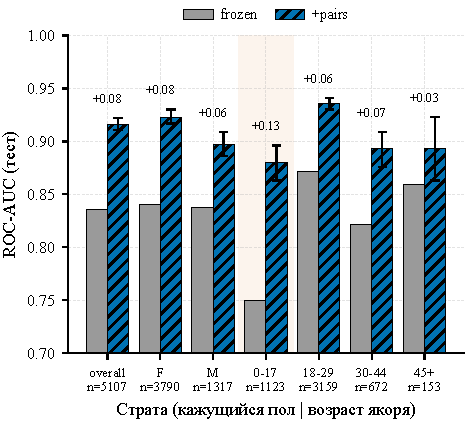
\includegraphics[width=\columnwidth]{fig_fairness_ru.pdf}
\caption{Аудит по кажущимся демографиям: frozen против $+$pairs (ROC-AUC) по стратам кажущегося
пола/возраста. Каждая страта улучшается; наибольший прирост — у младшей (0--17) группы. Усы — 95\%
парные bootstrap-ДИ прироста.}
\label{fig:fairness}
\end{figure}

При фиксированной операционной точке (поглобальный порог модели при 1\% FMR) $+$pairs снижает
false-non-match rate в \emph{каждой} кажущейся страте (0--17 $0.852\!\rightarrow\!0.656$, кажущ.-женский
$0.674\!\rightarrow\!0.509$, кажущ.-мужской $0.743\!\rightarrow\!0.534$), причём пострастовые наклоны
логистической калибровки равномерно положительны (9.0--11.7); единственное исключение — малая страта
45+, чей FMR рассеивается у глобального порога (шум выборки). Прирост child$\leftrightarrow$adult
подтверждается на независимом подмножестве FG-NET (одно фото до 13, другое после 25; 195 позитивов):
$+$pairs поднимает ROC-AUC $0.684\,[0.63,0.74]\!\rightarrow\!0.813\,[0.77,0.86]$ ($+$0.129,
непересекающиеся 95\% ДИ).

\section{Кросс-исходный и кросс-платформенный перенос}\label{sup:cross}
Табл.~\ref{tab:crossplatform} приводит VK-обученную модель, оценённую на независимом не-VK
Reddit-наборе «тогда/сейчас», а табл.~\ref{tab:crosssource} — двунаправленный перенос (backbone,
обученный \emph{только} на малом 220-личностном Reddit-источнике, тоже помогает на VK).

\begin{table*}[t]
\centering
\small
\begin{tabular}{@{}lcc@{}}
\toprule
Reddit (не-VK) тест-метрика & Frozen & $+$pairs (VK-обуч.) \\
\midrule
Общий ROC-AUC [95\% ДИ] & 0.718 [0.70, 0.74] & \textbf{0.749 [0.73, 0.77]} \\
EER & 0.345 & \textbf{0.328} \\
TAR@FAR$=$1\% & 0.271 & \textbf{0.279} \\
\midrule
Тест-пар (поз.\ / нег.) & \multicolumn{2}{c}{1{,}575 / 1{,}575} \\
\bottomrule
\end{tabular}
\caption{Кросс-платформенный перенос: VK-обученная модель на независимом Reddit (не-VK) наборе
«тогда/сейчас» (396 постов $\rightarrow$ 1{,}575 позитивных пар после фильтра многолюдных коллажей).}
\label{tab:crossplatform}
\end{table*}

\begin{table}[t]
\centering
\small
\setlength{\tabcolsep}{4pt}
\begin{tabular}{@{}llccc@{}}
\toprule
Обучение & Тест & Frozen & Дообуч. & $\Delta$ \\
\midrule
VK & Reddit (в целом) & 0.718 & 0.749 & $+$0.031 \\
Reddit & FG-NET 25+ & 0.736 & 0.783 & $+$0.047 \\
Reddit & VK внутр.\ 25+ & 0.640 & 0.659 & $+$0.019 \\
\bottomrule
\end{tabular}
\caption{Кросс-исходный перенос в обе стороны. Reddit$\to$VK — малый 220-личностный пилот, подтверждающий
неспецифичность источника, не headline-заявка.}
\label{tab:crosssource}
\end{table}

\section{Калибровка и майнинг трудных негативов}\label{sup:calib}
\textbf{Калибровка.} Сырой косинус (Platt) плохо откалиброван по бакетам разрыва — переуверен на 15--25
лет (ECE 0.052); калибратор $P(\text{один}\mid\text{косинус},\text{разрыв возраста})$ исправляет каждый
бакет (15--25 $\rightarrow$ 0.017) и улучшает общий Brier-score ($0.035\!\rightarrow\!0.029$), давая
пригодную, возраст-зависимую вероятность одной идентичности.

\textbf{Майнинг трудных негативов.} Добавление топ-5 наиболее похожих лиц других людей на якорь (в
трудной косинусной полосе, исключая диапазон near-duplicate/неопределённости) дополнительно обостряет
различение на большом разрыве (табл.~\ref{tab:hardneg}): FG-NET большой разрыв растёт до $0.868\pm0.004$
по трём сидам, но лёгкие бенчмарки забываются \emph{сильнее}, а общий ROC FG-NET падает. Трудные негативы
тем самым меняют точность на общих бенчмарках на разделение по большому разрыву — полезно для сценария
кросс-возрастного поиска, а не для универсального верификатора.

\begin{table}[t]
\centering
\small
\begin{tabular}{@{}lccc@{}}
\toprule
Метрика & Frozen & $+$pairs & $+$pairs$+$hard-neg \\
\midrule
FG-NET больш.\ разрыв & 0.736 & 0.848 & \textbf{0.868\,$\pm$\,0.004} \\
FG-NET ROC & 0.896 & 0.923 & 0.912\,$\pm$\,0.003 \\
LFW точность & 0.964 & 0.968 & 0.925\,$\pm$\,0.009 \\
AgeDB-30 ROC & 0.953 & 0.946 & 0.911\,$\pm$\,0.013 \\
CALFW ROC & 0.948 & 0.949 & 0.898\,$\pm$\,0.015 \\
\bottomrule
\end{tabular}
\caption{Майнинг трудных негативов (FaceNet, очищенные; внешние бенчмарки). $+$hard-neg — среднее $\pm$
std по трём сидам.}
\label{tab:hardneg}
\end{table}

\section{Утверждения против свидетельств}\label{sup:claims}
Табл.~\ref{tab:claims} сопоставляет каждое содержательное утверждение с его свидетельством и объёмом.

\begin{table*}[t]
\centering
\small
\begin{tabular}{@{}p{0.30\textwidth}p{0.40\textwidth}p{0.22\textwidth}@{}}
\toprule
Утверждение & Свидетельство & Объём / оговорка \\
\midrule
Добытые пары улучшают кросс-возрастную верификацию на большом разрыве & FG-NET больш.\ разрыв $0.736\!\rightarrow\!0.848$, непересекающиеся ДИ, DeLong $p<10^{-19}$ & слабые/средние backbone \\
Источник данных $>$ выбор цели & контрастив/ArcFace/CosFace совпадают (0.848/0.851/0.843); sub-center ничего не добавляет & среди проверенных целей \\
Реальные пары $>$ синтетич.\ старение & реал.\ 0.848 против согл.\ по разрыву FRAN 0.759; контроль нативного разрешения & этот протокол \\
Механизм — устранение возрастного shortcut & age-matched негативы обрушивают frozen до $\approx$0.52; $+$pairs восстанавливает до 0.838 & внутр.\ тест 25+ \\
Источник обобщается за платформу & VK$\to$Reddit $+$0.031; child$\leftrightarrow$adult FG-NET $+$0.129 & не платформо-агностично \\
Целевой, не универсальный прирост & сконцентрирован на подмножестве большого разрыва; лёгкие бенчмарки не меняются (LFW TAR@0.1\% $0.814\!\rightarrow\!0.816$) & объём — поиск на большом разрыве \\
$\approx$половина сырых позитивов была near-duplicate & $-$52\% числа позитивов, стабильно по дедупу 0.93--0.97 & находка очистки \\
\bottomrule
\end{tabular}
\caption{Карта «утверждения против свидетельств».}
\label{tab:claims}
\end{table*}

\section{Карточка модели и данных}\label{sup:card}
\textbf{Назначение.} Исследование кросс-возрастного сопоставления личности на основе согласия; модель
выдаёт кандидатов для проверки человеком, а не автоматическое решение. \textbf{Вне объёма:} массовая
идентификация, слежка, деанонимизация, любая обработка данных несовершеннолетних без правовой основы.
\textbf{Обучающие данные.} Два публичных «тогда/сейчас» VK-сообщества (одна платформа, русскоязычный
контекст); смещение к кажущемуся женскому полу (76.7\%); разреженность при кажущемся возрасте 45+; слабая
супервизия одного человека из со-встречаемости в одном посте с LLM-разобранными возрастами подписей как
вторичным сигналом. \textbf{Данные оценки.} LFW, AgeDB-30, CALFW, FG-NET (и его подмножества большого
разрыва и child$\leftrightarrow$adult), внутренний очищенный кросс-возрастной тест и независимый не-VK
Reddit-набор «тогда/сейчас». \textbf{Метрики.} ROC-AUC (беспороговая; основная), EER, TAR@FAR и
пострастовая калибровка. \textbf{Этические соображения.} Чувствительные биометрические данные; сырые
лица/посты не публикуются; веса/эмбеддинги предоставляются по запросу в рамках краткого соглашения об
исследовательском использовании; обезличенный набор данных доступен по запросу (формальная документация
при необходимости); несовершеннолетние исключены при отсутствии правовых рамок; DPIA и карточка
датасета~\cite{gebru2021datasheets} сопровождают релиз. \textbf{Оговорки.} Прирост сконцентрирован на большом разрыве (лёгкие бенчмарки не меняются); сосредоточен в слабых/средних backbone; кажущиеся (не
самоидентифицированные) атрибуты; супервизия проверена, но не сертифицирована.

\section{Детали воспроизводимости}\label{sup:repro}
\textbf{Конвейер.} Фильтрация \emph{пригодных лиц} (det-score, минимальный размер, размытие по Лапласу,
единственная цель); детекция/выравнивание InsightFace \texttt{buffalo\_l} RetinaFace $+$ 5-точечный
ArcFace \texttt{norm\_crop} (112\,px; вход FaceNet 160\,px); эмбеддинги ArcFace \texttt{w600k\_r50} для
кластеризации (union-find, косинус $\geq$ 0.85) и дедупа (косинус $\geq$ 0.97); LLM с версионированными
кэшированными промптами для разбора возраста и целостности групп; сплит по человеку 70/15/15 (сид 42,
сбалансированные негативы, плюс вариант с age-matched негативами). \textbf{Обучение.} Дообучение головы
с margin-контрастивной потерей (lr 3e-5 слабые / 1e-5 сильные; ранняя остановка по val-AUC; сиды 42/1/2);
margin-цели классификации идентичности (ArcFace/CosFace/SphereFace и sub-center ArcFace с $K{=}3$) для
сравнения целей; ROC-AUC/EER/TAR@FAR на чистом NumPy. \textbf{Вычисления.} Всё исследование выполняется
на одном ноутбуке: одна NVIDIA RTX~3060 Laptop GPU (6\,ГБ), AMD Ryzen~7~5800H (8C/16T) и 16\,ГБ ОЗУ под
Windows~11; Python~3.12, PyTorch~2.12 (CUDA~13.2), InsightFace~1.0 / ONNX~Runtime~1.26, scikit-learn~1.9,
Matplotlib~3.11. \textbf{Доступность.} Код, конфигурации, версионированные LLM-промпты, замороженные
сплиты (по хешу) и обезличенный протокол бенчмарка публикуются; сырые изображения лиц и посты не
публикуются, поэтому воспроизведение майнинга частично (мы публикуем кэшированные выходы LLM для
детерминированного replay). Заполненный чек-лист воспроизводимости прилагается к подаче.

\bibliographystyle{IEEEtran}
\bibliography{../../../shared/refs}

\end{document}
